\documentclass[titlepage,12pt]{article}

\usepackage[T2A]{fontenc}
\usepackage[utf8]{inputenc}  

\usepackage{amsmath}
\usepackage{amssymb}
\usepackage{graphicx}
\renewcommand{\figurename}{Рис.}

\oddsidemargin = 0.6cm
\textwidth = 16cm
\textheight = 21cm
\headheight = 0cm
\sloppy

\author{Кочуркин Иван Алексеевич \\ Группа ИУ7-92 \\ Вариант \textnumero 11}
\title{Отчёт по лабораторной работе \textnumero 3 \\по курсу\\ Методы вычислений}
\date{2011 г.}

\begin{document}

\maketitle

\setcounter{page}{2}
\newpage
\section{Постановка задачи}
\subsection{Краевая задача}

\begin{align*}
&\frac{\partial^2 u}{\partial x^2} + \frac{\partial^2 u}{\partial y^2} = -f(x,y), \quad 0 \leqslant x \leqslant a, 
	\quad 0 \leqslant y \leqslant b\\
&u|_{x=0} = \varphi_0(y) \qquad u|_{x=a} = \varphi_a(y)\\
&u|_{y=0} = \psi_0(x) \qquad u|_{y=b} = \psi_b(x)
\end{align*}


\subsection{Исходные данные}
\begin{enumerate}
	\item{Размеры области решения $a = 1$, $b = 1$}
	\item{$\varphi_0 (y) = y$, \quad $\varphi_a (y) = y^2$}
	\item{$\psi_0 (x) = 2x(1-x)$, \quad $\psi_b (x) = 1$}
	\item{$f(x,y) = 0$}
\end{enumerate}

\section{Решение}
\subsection{Разностные уравнения}
На заданом поле решения выбирается сетка из N равноотстоящих узлов по каждой координате.\par

\begin{align*}
&\frac{u_{i-1,j} - 2u_{i,j} + u_{i+1,j}}{h_x^2} + \frac{u_{i,j-1} - 2u_{i,j} + u_{i,j+1}}{h_y^2} = -f(x_i,y_j) \\ 
&u_{1j} = \varphi_0(y_j), u_{Nj} = \varphi_a(y_j), u_{i1} = \psi_0(x_i), u_{iN} = \psi_b(x_i)\\
&\qquad \text{, где } i = \overline{1,N-1},\quad	j = \overline{1,N-1}
\end{align*}

Выбранная схема является абсолютно устойчивой, поэтому нет ограничений на выбор шагов по переменным. Шаг влияет исключительно на величину невязки при счёте. Использованы шаги $h_x = \frac{a}{N}, h_y = \frac{b}{N} , N = 80$.

\subsection{Метод верхней релаксации}
Для решения получившейся СЛАУ используется итерационный метод верхней релаксации. В координатной форме для нашей СЛАУ он выглядит так:
\begin{align*}
&u_{ij}^{k+1/2} = \frac{h_y^2}{2(h_x^2 + h_y^2)}(u_{i-1,j}^{k+1} + u_{i+1,j}^k) + 
	  							\frac{h_x^2}{2(h_x^2 + h_y^2)}(u_{i,j-1}^{k+1} + u_{i,j+1}^k) +
								  \frac{h_x^2 h_y^2}{2(h_x^2 + h_y^2)} f_{ij} \\
&u_{ij}^{k+1} = \omega u_{ij}^{k+1/2} + (1-\omega)u_{ij}^k
\end{align*}

Величина параметра метода релаксации влияет на скорость его сходимости. Оптимальным является значение:
$$
\omega_{opt} = \frac{2}{1+\sin\dfrac{\pi}{N-1}}
$$

Если на выходе требуется, чтобы выполнялось $\|u^{k+1}\|_1 < \epsilon$, итерации метода прекращаются при выполнении следующего условия:
$$
\|u^{k+1} - u^k\|_1 < (2-\omega)\epsilon
$$

\subsection{Устойчивость разностной схемы}
Данная разностной схемы является устойчивой. 

\subsection{Порядок аппроксимации разностной схемы}
Аппроксимация разностной схемы "Крест" оценивается как $O(h_x^2 + h_y^2)$. 

\subsection{Определение ошибки}
Для определения ошибки воспользуемся формулой Рунге 
$$
z^I \approx \frac{|u^I - u^{II}|}{r^2-1}
$$
один раз, приняв $r=2$. При этом используется обычная сетка $\omega^I$ с шагами $\tau$ и $h$ и сгущённая сетка $\omega^{II}$.Поскольку порядок аппроксимации счёта по переменным одинаковый, шаги у сгущённой сетки $\omega^{II}$ будут соответственно $h_x / r$ и $h_y / r$. Формула применяется для совпадающих узлов двух сеток.\par
Результаты: максимальная погрешность  $z^I_{max} = 0.101354$, среднее значение погрешности $\overline{z^I} = 0.025783$.

\begin{figure}[h]
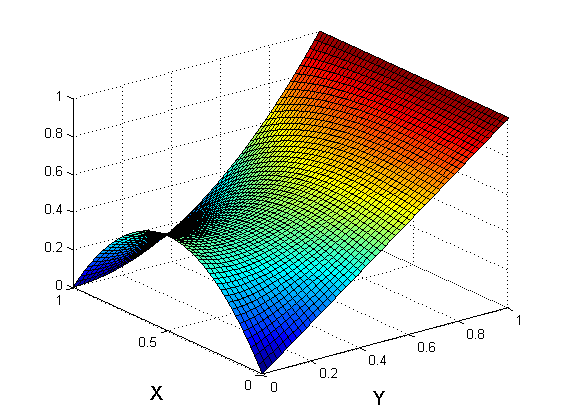
\includegraphics[width = 16cm]{Screen.png}
\caption{График функции}
\label{fig:16}	
\end{figure}

\end{document}
